\documentclass[a4paper,12pt]{report}
\usepackage{algorithmic}
\usepackage[linesnumbered,ruled,vlined]{algorithm2e}
\usepackage[margin=2cm]{geometry}
\usepackage[utf8]{inputenc}
\usepackage{listings} 
\usepackage{graphicx} 
\usepackage{color}
\usepackage{xcolor}
\usepackage{hyperref}
\usepackage{verbatim}
%\usepackage{mdframed}

\newcommand{\currentdata}{14 February 2015}
\newtheorem{example}{Example}

\begin{document}
\vspace{-5cm}
\begin{center}
Department of Computer Science\\
Technical University of Cluj-Napoca\\

\includegraphics[width=10cm]{fig/footer}
\end{center}
\vspace{1cm}
%\maketitle
\begin{center}
\begin{Large}
 \textbf{Artificial Intelligence}\\
\end{Large}
\textit{Laboratory activity}\\
\vspace{3cm}
Name: Fodor, Zsofia and Katona, Áron\\
Group: 30433\\
Email: fodorzsofi@yahoo.com katonaaron01@gmail.com\\
\vspace{12cm}
Teaching Assistant: Adrian Groza\\
Adrian.Groza@cs.utcluj.ro\\
\vspace{1cm}

\includegraphics[width=10cm]{fig/footer}
\end{center}

\tableofcontents

\chapter{Bidirectional Search} 

Bidirectional search simultaneously searches from the start state to the goal state (\textbf{forward searching}) and from the goal state to the start state  (\textbf{backward searching}) hoping that these two searches will meet. The time and space complexity was reduced from $O(b^d)$ to $O(2 * b^{d/2}) = O(b^{d/2}) << O(b^d)$, where $b$ is the branching factor and $d$ is the depth of the shallowest solution.

\section{Implementation}


The algorithm uses the \textbf{Breadth-First Search policy}, meaning that it takes the shallowest node first. It stops when the forward and backward search intersect. If no solutions is found, than it returns \textit{None}.

We used two sets one representing the explored nodes that are still in the queue and another one, that contains the visited nodes that were popped out of the queue.
Entering the while loop, we firstly analyze the forward search. Take the next node from the corresponding queue and if it is not yet visited we put it in the visited set. After we have iterated through the nodes of the backward search, if there is a meeting point then we return the current path and the path accumulated by the backward search in reverse order.

Next we analyze the backward search the same way as we did for the forward search, the only difference being that we replace each action with its opposite action, we reverse the list containing them and add it to the accumulated path.

The motivation behind using sets is that they are more efficient than lists in verifying whether they contain an arbitrary element.

Source code: Appendix \ref{sec:code_bs}.

\begin{figure}[ht]
    \centering
    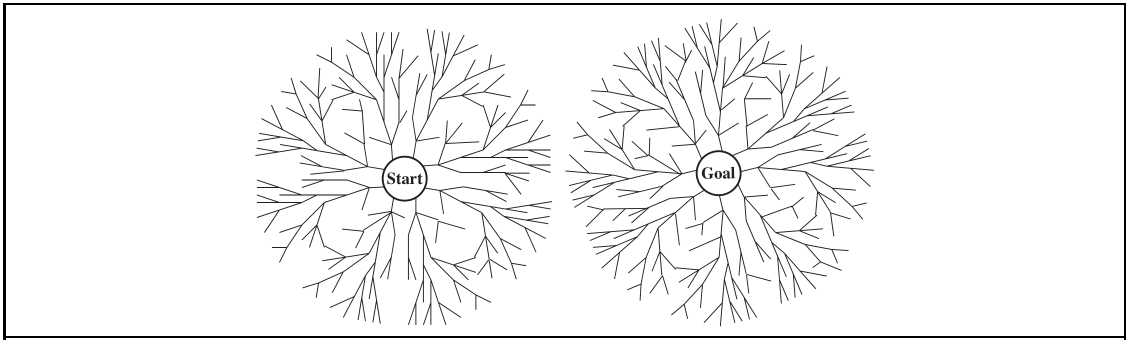
\includegraphics[width=.8\linewidth]{fig/bs.png}
    \caption{Visualization of the bidirectional search algorithm. \cite{aima2020}} 
    \label{fig:bs}
\end{figure}


\chapter{Iterative Deepening Depth-First Search} 

\section{Depth-Limited Search}
\label{sec:dls}

The depth-limited search is similar to the depth-first search, with the only difference, that a \textbf{depth bound} is added. Thus the algorithm searches for the goal state until the search tree's depth reaches the bound. If the bound is reached, the search backtracks to the parent node and continues searching in the next successor of the parent node. Therefore if there is a path to the goal, whose length is smaller than or equal to the bound, it will be found.

\subsection{Implementation}

To represent the nodes we used the \verb|Node| class, which is a simple data class whose \verb|state|,\verb|action| and \verb|cost| fields are used. More information about the class can be found in Appendix \ref{sec:nodes}.

The algorithm is a modified version of the recursive \textbf{depth-first search}. At each level of recursion, the function calls itself for all of the successors. The function returns not only the found goal node on success and None on error, but also an additional boolean parameter which specifies whether the search terminated because of a cutoff, or not. In each level of recursion, the limit is decremented. When it reaches 0, the returned cutoff value is true.

Source code: Appendix \ref{sec:code_dls}.


\section{Iterative Deepening Search}

The iterative deepening search strategies apply a search algorithm multiple times, with increasing bounds until the goal is reached. The calculation of the bound depends on the applied algorithm. We used the strategy of iterative deepening for the following search algorithms: depth-first search (\ref{sec:iddfs}) and A* (\ref{sec:idastar}).


\section{Iterative Deepening Depth-First Search}
\label{sec:iddfs}

Starting from an initial bound of 0, we call the depth-limited search and verify the returned result. In case a cutoff occurred, we increase the bound by one, and start again the search. If the goal node was found, the path from the start node which ends in the goal node is reconstructed and returned.

The algorithm is complete, because depth-first search, and in particular depth-limited search is guaranteed to find a solution, if the distance to the goal node is inside the bound. The bound is incremented from 0 indefinitely, thus if the solution exists, it will be found. 

The algorithm is optimal for unit action costs, because if no solution was found for bound $b$, the length of the shortest path from the start node to the goal node is at least $b+1$, and if there is any solution with length $b+1$, all of them are optimal solutions, and one of them will be found by the depth-limited search.

Source code: Appendix \ref{sec:code_iddfs}.



\documentclass{report}
\usepackage[utf8]{inputenc}



\begin{document}

\chapter{Iterative Deepening A* Search}

Iterative deepening is a preferred algorithm when we have a larger search state space than the one that can fit in memory and the depth of our solution is not known. 

Iterative Deepening A* is similar to A* the difference being that we do not keep all reached states in memory, at a cost of visiting some states multiple times. It is a very frequently used algorithm for problems that do not fit in memory, as stated above.

\section{Implementation}

The idea behind the algorithm was that we search the node with the lowest combined cost and heuristic first (\textbf{f = g + h}). The algorithm is limiting the size of the frontier by using this calculated f value as a bound.

We used a set in which we stored the visited nodes. Searching in sets is faster than searching in lists, that is why we chose set.
Besides this set, we used a list called path, that stored for each node its state, the action that needs to be performed to get there from the previous node and the cost.

We have a utility function that we call repeatedly until the returned value is either a very large number ($\infty$)  or  the \textit{None} state and we change the value of the bound to the returned value if none of these conditions is satisfied. 

The utility function begins with taking the last element from the path, computing the f value of this element and comparing it to the bound. If it is larger than the bound, we return the f value. If the state of the node is the goal state, it means we reached our goal, so we return the \textit{None} state. If none of these conditions are fulfilled, then we iterate through each child of the current node, add it to the visited set and to the path list, then we call the utility function on it. We make the adjustments according to the returned value of this call, remove the node from the visited list and the path. 
Lastly we return the minimum value which represents the minimum cost of all values that exceeded the current bound. 

\section{Remarks}

This algorithm was actually easy to implement after we understood the idea behind it. 

Comparing the number of expanded nodes we can see that it is much larger than for the A* algorithm, because of the fact that we do not keep all reached states in memory risking the fact that we might visit some nodes more than once. 


\end{document}

\chapter{Recursive Best-First Search} 

The recursive best-first search, similarly to the depth-limited search (\ref{sec:dls}), searches for the deepest node first, but stops after surpassing a bound. But in this case the bound is placed on the f-value of a node, instead of its depth.

The f-value of a node is the maximum between the f-value of its parent and the cost of reaching the node + the heuristic, i.e. $f(n) = max\{ g(n) + h(n), f(n.parent) \}$. When a branch of the search is cut off because the limit on the f-value, while backtracking, the f-value of a parent node will be updated with the f-value of its child. This way, the f-value of a node will become a more and more accurate estimation of the true cost of reaching the goal node from it.

This algorithm uses the principle of best-first searching. It only expands the node with the smallest f-value. If the node is on the current searching branch, than it will be expanded, otherwise the search tree backtracks to the level of the node with the smallest f-value. Therefore at each level of recursion we take the first two successors with the lowest f-value, call the search for the best option, and supply the bound as the f-limit of the alternative successor. This is repeated until the solution is found, or until the f-value of the best node will become greater than the f-limit. Thus it always considers a best and an alternative path, and switches between them, if the alternative path becomes the best one, in terms of lowest f-value.

The advantage of this algorithm is that it uses linear space: used for storing the nodes along the search path, and also the sibling of each node. The disadvantage is that it regenerates already visited nodes, which could happen very frequently. Thus it trades speed for storage.

For the implementation the \verb|Node| class (\ref{sec:nodes}) was used for storing the nodes, and a priority queue was used for obtaining the best successor of a node. The recursive function returns the result and None, if the goal node was found. If the goal was not found, it returns None and the f-value of the deepest node reached before surpassing the limit.

Source code: Appendix \ref{sec:code_rbfs}.

\begin{figure}[ht]
    \centering
    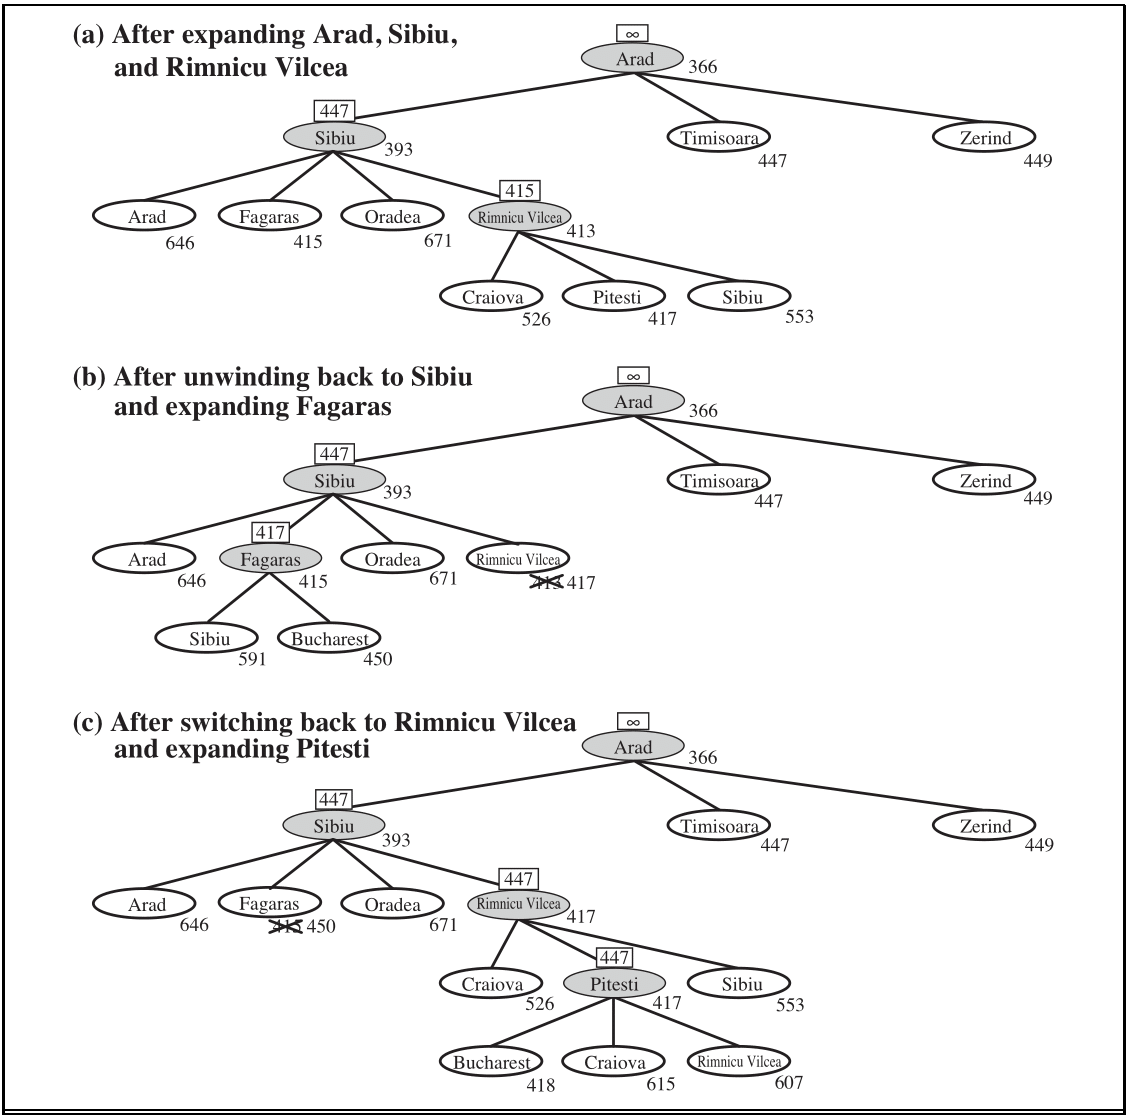
\includegraphics[width=\linewidth]{fig/rbfs.png}
    \caption{Finding a path from Arad to Bucharest by using recursive best-first search. The number above a node is its f-limit, and the number on the right of it is its f-value. The searching branch was switched two times. \cite{aima2020}} 
    \label{fig:rbfs}
\end{figure}




\bibliographystyle{plain}
\bibliography{is}

\appendix

\vspace{2cm}
\begin{center}
Intelligent Systems Group\\

\includegraphics[width=10cm]{fig/footer}
\end{center}



\end{document}
